\section{Motivating Example}
\label{sec:motiv}
% \todo{prettify text}
To understand the goal and the potential of our solution, consider the case of the ASCAs attack shown in Figure~\ref{fig:example}.

The first line displayed in Figure~\ref{fig:example} represents the text typed by the victim. Most works on the literature consider non-noisy scenarios; thus, this same text is recovered, which makes them claim high recovery rates. In noisy scenarios, however, the recovered text will be similar to the one displayed in the second line of Figure~\ref{fig:example}, which explains why most works fail in recovering the text in these scenarios. Ideally, we would like to have a correction mechanism that allows this text to be mapped back to the original text as much as possible, as shown in the last line. 

\begin{figure}[htbp]
    \centering
    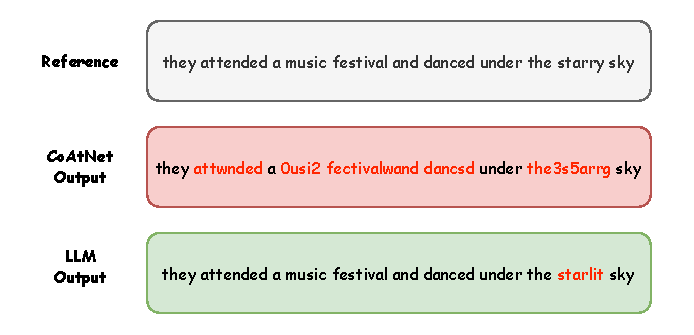
\includegraphics[width=\columnwidth]{images/figure_error_correction_example.pdf}
    \caption{Example of Error Detection and Correction Using LLMs: The initial text sequence (top) represents the ideal output. The noisy prediction (middle) introduces typographical and semantic errors due to environmental noise or model inaccuracies. The corrected output (bottom) demonstrates how LLMs refine the sequence using contextual understanding, substituting errors (e.g., \textit{attwnded} to \textit{attended}).}
    \label{fig:example}
\end{figure}

While textual examples illustrate the impact of noise, it is also insightful to visualize the differences at the signal level.Figure~\ref{fig:compare} presents two Mel spectrograms of the same keystroke—specifically, the digit ``0'' from the phone dataset—one in a clean setting and the other in a noisy setting. The spectrogram on the left corresponds to the clean scenario, where the keystroke exhibits distinct frequency characteristics. On the right, background noise distorts these features, making classification significantly harder. This visual evidence supports our argument that a robust classification and correction mechanism is necessary to achieve reliable text recovery in real-world settings.

\begin{figure}[htbp]
    \centering

    % Clean and Noisy Spectrograms
    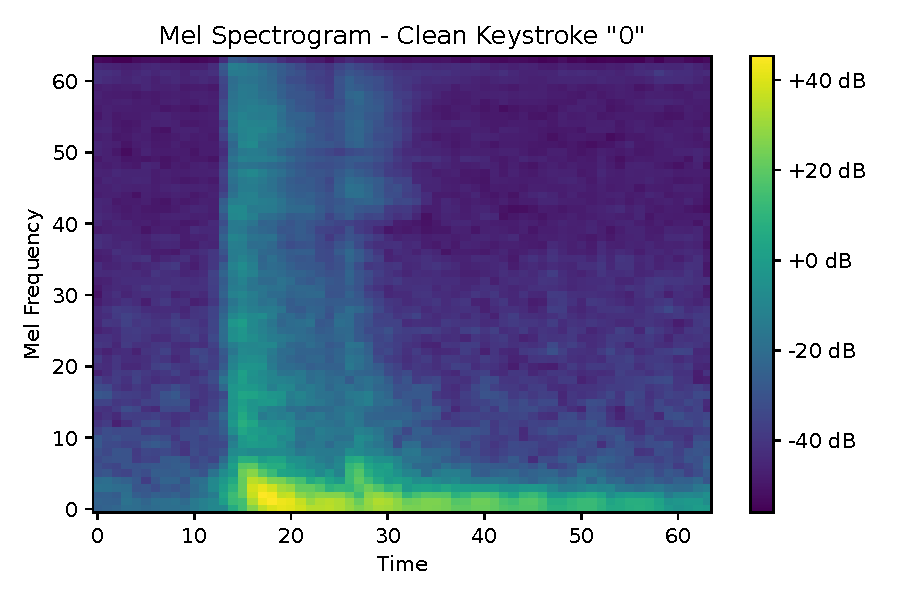
\includegraphics[width=0.50\columnwidth]{images/spectrogram_clean.pdf}\hfill
    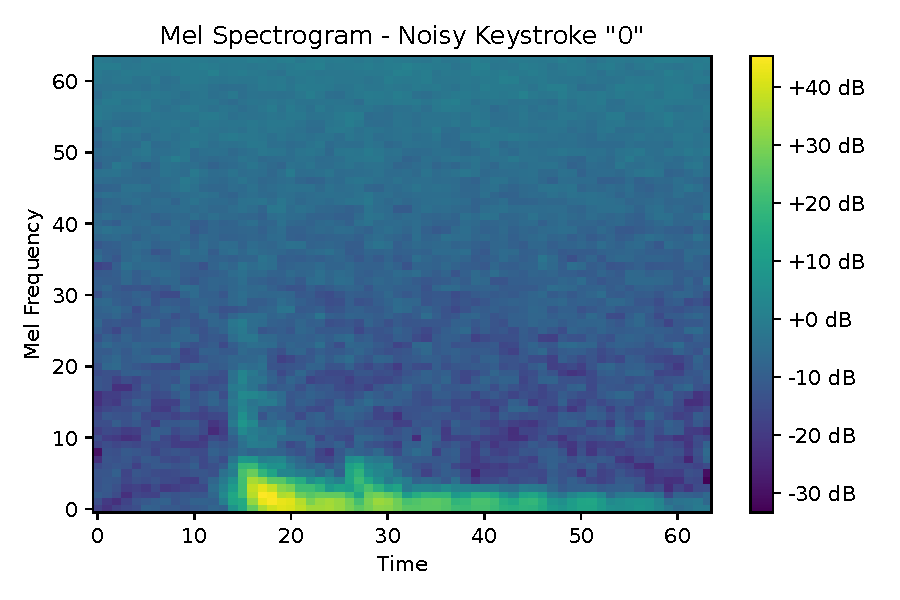
\includegraphics[width=0.50\columnwidth]{images/spectrogram_noisy.pdf}

    \caption{Comparison of Mel spectrograms for the keystroke corresponding to digit ``0'' from the phone dataset in a clean (left) and noisy (right) scenario. The noisy spectrogram exhibits additional artifacts that distort and attenuate the keystroke's spectral features, reducing the signal energy and making classification significantly more challenging.}
    \label{fig:compare}
\end{figure}

These presented examples were obtained by applying the proposed tool to the reference benchmark, which positions our solution closer to the ideal scenario than the previous related works. This demonstrates the effectiveness of our approach in handling noisy conditions, ensuring higher accuracy in text recovery. The following sections describe how this result can be achieved.